%%%%%%%%%%%%%%%%%%%%%%%%%%%%%%%%%%%%%%%%%
% Memo
% LaTeX Template
% Version 1.0 (30/12/13)
%
% This template has been downloaded from:
% http://www.LaTeXTemplates.com
%
% Original author:
% Rob Oakes (http://www.oak-tree.us) with modifications by:
% Vel (vel@latextemplates.com)
%
% License:
% CC BY-NC-SA 3.0 (http://creativecommons.org/licenses/by-nc-sa/3.0/)
%
%%%%%%%%%%%%%%%%%%%%%%%%%%%%%%%%%%%%%%%%%

\documentclass[letterpaper,11pt]{texMemo} % Set the paper size (letterpaper, a4paper, etc) and font size (10pt, 11pt or 12pt)

\usepackage{parskip} % Adds spacing between paragraphs
\usepackage[colorlinks]{hyperref}
\usepackage{graphicx}
\usepackage{float}
\usepackage{hyperref}
\hypersetup{citecolor=DeepPink4}
\hypersetup{linkcolor=red}
\hypersetup{urlcolor=blue}
\usepackage{cleveref}
\setlength{\parindent}{15pt} % Indent paragraphs

%----------------------------------------------------------------------------------------
%	MEMO INFORMATION
%----------------------------------------------------------------------------------------

\memoto{Dr.Randy Hoover} % Recipient(s)

\memofrom{Benjamin LeBrun, Benjamin Garcia} % Sender(s)

\memosubject{Lab Assignment 5: Timers and Motor Control} % Memo subject

\memodate{\today} % Date, set to \today for automatically printing todays date

% \logo{\includegraphics[width=0.1\textwidth]{logo.png}} % Institution logo at the top right of the memo, comment out this line for no logo

%----------------------------------------------------------------------------------------

\begin{document}

\maketitle % Print the memo header information

%----------------------------------------------------------------------------------------
%	MEMO CONTENT
%----------------------------------------------------------------------------------------

\section*{Introduction}
For this lab, we utilized the full car kit of our Elegoo robot package to 
explore using power width modulation (PWM) to send a controlled motor signal to an H-bridge chip
and drive a set of DC motors with two separate channels. This required the
use of writing to the Atmega328p's internal timers to prevent overloading or locking
the CPU with delay signals or other inefficient methods.

\section*{Equipment}
While the lab used the entire robot kit assembled together, the primary devices
we used were:

\begin{itemize}
    \item Acrylic vehicle body with screws, assembled
    \item Elegoo Uno (chip: Atmega328p)
    \item 4 DC motors with wheels, screws 
    \item L298 H bridge module dual channel
    \item 2 ICR18650 batteries with battery box
    \item Ribbon cables
    \item Host laptop with AVR-gcc 8-bit toolchain
    \item USB 2.0 A to B cable
\end{itemize}

\subsection*{Configuration}
Our robot vehicle was assembled according to Elegoo's instructions which can be found
on Elegoo's website at \url{https://www.elegoo.com/download/}. For this lab, we are
using the V3.0 version of the robot kit.

The components in the kit have a clearly marked port on the Arduino shield included in 
the package. This makes it easier to identify and connect together ports using the also 
included ribbon cables with some degree of cable management. One of the early pitfalls is
that the H bridge connector is a six pin ribbon cable, which to the uncareful eye looks like 
the five pin cable connector between the shield board and the line following IR sensors.

Besides the ribbon cable for our ports, we also have a DC cable to power the H bridge driver. 
This is because the DC motors have massively larger power requirements (up to a maximum of 2 amps) 
than our Arduino (40 milliamps maximum, both at 5 volts). Therefore, the external batteries are 
required to power the DC motors via the H bridge separate from the Arduino. Wheels were also attached 
and secured with standard phillips head screws.

\begin{figure}[!ht]
\begin{center}
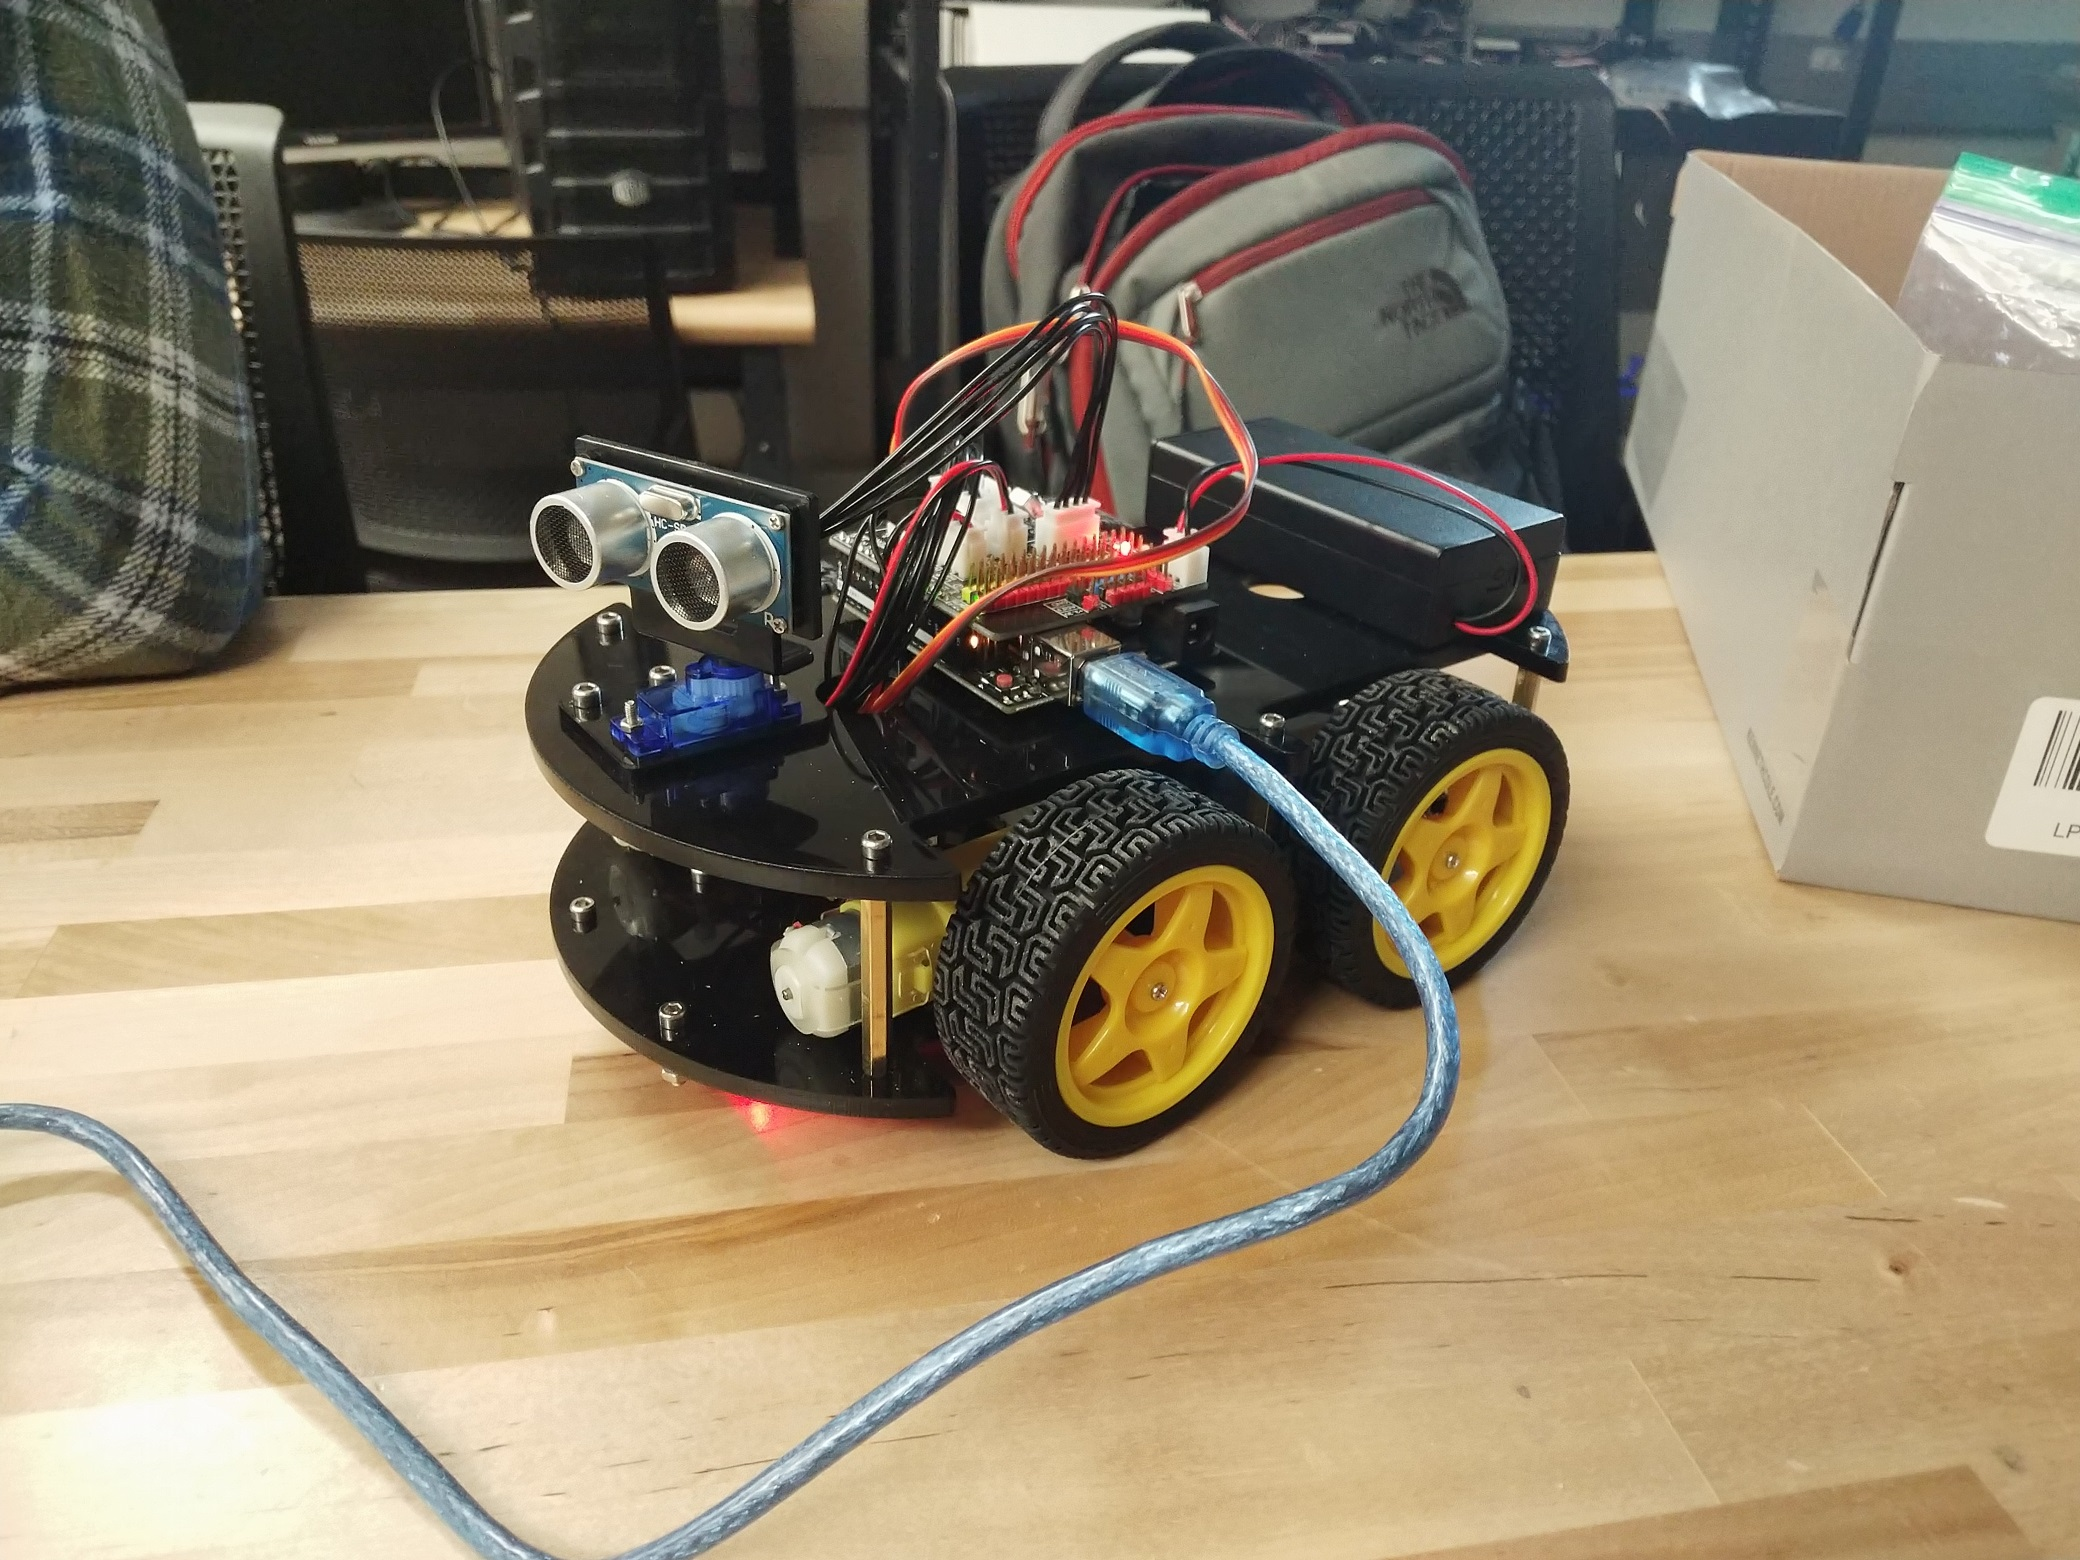
\includegraphics[width=\linewidth]{spare_me.jpg}
\end{center}
\caption{Fully assembled Elegoo robot car kit V3.0.}
\label{fig:f4}
\end{figure}

\section*{Implementation}
For this lab we are writing our own motor driver header and 
library which should allow us to use in the future. Because 
it also uses a pin map header file, we can also move the motor
headers around when needed.




\section*{Discussion}
Discuss challenges met in completion of the lab and how you solved them. Communicate what you learned from the lab, and comment on where this lab material would be applicable 'in the real world'. 

\section*{Responses}
Respond intelligently and at necessary length to any questions posed in the lab assignment.
\begin{enumerate}
\item Enumerations are a useful for addressing specific questions.
\end{enumerate} 

\section*{Appendices}
You'll want to put your full code here, possibly datasheets. Each appendix should start on a fresh page. Check out the \textbf{lstlisting} package, it might make your life easier. 
\newpage

\section*{Appendix A: Nothing}

%----------------------------------------------------------------------------------------

\end{document}
\grid
